\chapter{\label{results}PID Controller using Multisim}


\section{Multisim}
NI Multisim (formerly MultiSIM) is an electronic schematic capture and simulation program which is part of a suite of circuit design programs, along with NI Ultiboard. Multisim is one of the few circuit design programs to employ the original Berkeley SPICE based software simulation. Multisim was originally created by a company named Electronics Workbench Group, which is now a division of National Instruments. Multisim includes microcontroller simulation (formerly known as MultiMCU), as well as integrated import and export features to the printed circuit board layout software in the suite, NI Ultiboard.

Multisim is widely used in academia and industry for circuits education, electronic schematic design and SPICE simulation. 

Multisim has desktop-based and browser-based editing environment. I used the browser-based editing environment to build the PID controller. 

\section{Circuit design}
\begin{figure}
	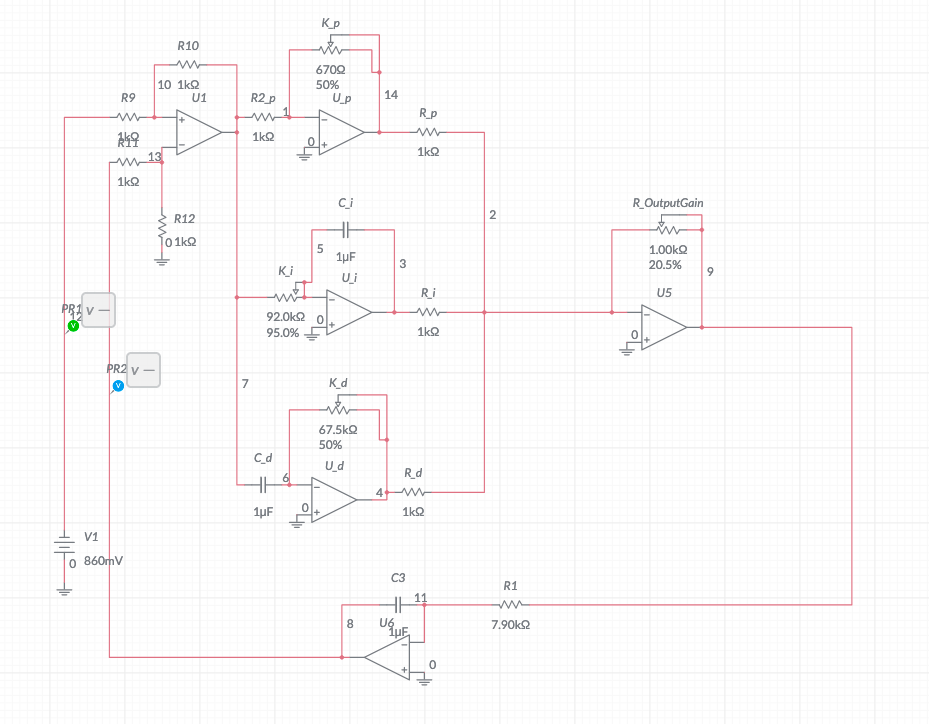
\includegraphics[width = \textwidth]{circuit.png}
	\caption{Circuit diagram drawn in multisim}
\end{figure}

 In this simulation we used 6 OPAMP. Three are used for integration differentiation and proportional amplification. One is used to calculate the difference between current value and the target value. Using one OPAMP wish you let a heater( this is a OPAMP as an amplifier.) At last we used one OPAMP for amplifying the sumed signal from all the integration differentiation and proportional circuit. 


 \subsection{Difference amplifier}
  the 0PAMP we used for this is labled U1 and has resistance $R_9 = 1K\Omega$  $R_10= 1K\Omega$. There for its amplification is one, in other words it's just calculating the difference between the signals. The signals we are feeding in this difference in the fire is the target signal and the current value. The output of this is going in integration circuit, differentiation circuit and proportional circuit.
 \subsection{Integration amplifier }
 The OPAMP we used for this is labled with $U_i$ and has resistance $K_i = 92K\Omega$ and camapciter $C_i = 1\mu F$  it has amplification of $K_i = 1.08E1$.
 \subsection{Differentiation amplifier}
 The OPAMP we used for this is labled with $U_d$ and has resistance $K_d = 67.5K\Omega$ and camapciter $C_i = 1\mu F$  it has amplification of $K_i = - 6.75E-2$.
 \subsection{Proportional amplifier}
 The OPAMP we used for this is labled with $U_p$ and has resistance $K_p = 670K\Omega$ and $R_p = 1K\Omega$  it has amplification of $K_p = 0.670$.
 \subsection{Amplification over sum}
 The OPAMP we used for this is labled with $U_5$ and has resistance $R_{OutputGain} = 1.0K\Omega$ and $R = 1K\Omega$  it has amplification of one.
 \subsection{Heater circuit simulation}
 The OPAMP we used for this is labled with $U_6$ and has resistance $R_1 = 7.9K\Omega$ and camapciter $C_i = 1\mu F$  it has amplification of $K_i = 1.26E2$.



 \section{Op-amp as Integrator}
 Operational amplifiers can be used for mathematical applications such as Integration and Differentiation by implementing specific op-amp configurations.

When the feedback path is made through a capacitor instead of a resistance , an RC Network has been established across the operational amplifiers’ negative feedback path. This kind of circuit configuration producing helps in implementing mathematical operation, specifically integration, and this operational amplifier circuit is known as an Operational amplifier Integrator circuit. The output of the circuit is the integration of the applied input voltage with time.
\begin{figure}[H]
	\includegraphics[width = 0.5\textwidth]{Opemp as I.png}
	\caption{OPAMP as integrator}
\end{figure}

\begin{figure}[H]
	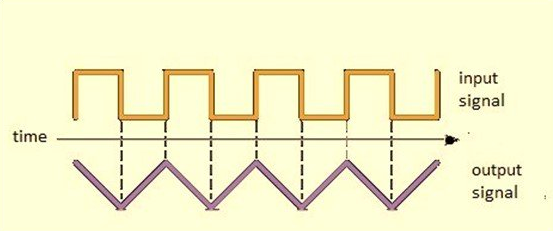
\includegraphics[width = 0.5\textwidth]{Inpput and output singal.png}
	\caption{input and output signal through OPAMP has an integrator.}
\end{figure}
Integrator circuits are basically inverting operational amplifiers (they work in inverting op-amp configuration, with suitable capacitors and resistors), which generally produce a triangular wave output from a square wave input. Hence, they are also used for creating triangular pulses.

The current in the feedback path is involved in the charging and discharging of the capacitor; therefore, the magnitude of the output signal is dependent on the amount of time a voltage is present (applied) at the input terminal of the circuit.

\subsection{Derivation of Op-amp as integrator}


As we know from the virtual ground concept, the voltage at point 1 is $0 \mathrm{~V}$. Hence, the capacitor is present between the terminals, one having zero potential and other at potential $\mathrm{V}_{0}$. When a constant voltage is applied at the input, it outcomes in a linearly increasing voltage (positive or negative as per the sign of the input signal) at the output whose rate of change is proportional to the value of the applied input voltage.
From the above circuitry it is observed, $V_{1}=V_{2}=0$
The input current as:
$$
\mathrm{I}=\frac{\mathrm{V}_{\mathrm{i}}-\mathrm{V}_{1}}{\mathrm{R}_{1}}=\frac{\mathrm{V}_{\mathrm{i}}}{\mathrm{R}_{1}}
$$
Due to the op-amp characteristics (the input impedance of the op-amp is infinite) as the input current to the input of an op-amp is ideally zero. Therefore the current passing from the input resistor by applied input voltage $\mathrm{V}_{\mathrm{i}}$ has flown along the feedback path into the capacitor $\mathrm{C}_{1}$.
Therefore the current from the output side can also be expressed as:
$$
\mathrm{I}=\mathrm{C}_{1} \frac{\mathrm{d}\left(\mathrm{V}_{1}-\mathrm{V}_{0}\right)}{\mathrm{dt}}=-\mathrm{C}_{1} \frac{\mathrm{d}}{\mathrm{dt}}\left(\mathrm{V}_{0}\right)
$$
Equating the above equations we get,
$$
\frac{\mathrm{V}_{\mathrm{i}}}{\mathrm{R}_{1}}=-\mathrm{C}_{1} \frac{\mathrm{d}}{\mathrm{dt}}\left(\mathrm{V}_{0}\right)
$$
Therefore the op-amp output of this integrator circuit is:
$$
\mathrm{V}_{0}=-\frac{1}{\mathrm{R}_{1} \mathrm{C}_{1}} \int_{0}^{t} \mathrm{~V}_{\mathrm{i}} \mathrm{dt}
$$
As a consequence the circuit has a gain constant of $-1 / \mathrm{RC}$. The negative sign point toward an $180^{\circ}$ phase shift.

\section{Op-amp as a Differentiator}
As we have studied earlier in the integrator circuit, op-amps can be used for implementing different mathematical applications. Here we will be studying the differential op-amp configuration in detail. The differentiator amplifier is also used for creating wave shapes and also in frequency modulators.

An operational amplifier differentiator basically works as a high pass filter and, the amplitude of the output voltage produced by the differentiator is proportionate to the change of the applied input voltage.

When the input resistance in the inverting terminal is replaced by a capacitor, an RC Network has been established across the operational amplifiers’ negative feedback path. This kind of circuit configuration helps in implementing differentiation of the input voltage, and this operational amplifier circuit configuration is known as an Operational amplifier differentiator circuit.

In a differentiating op-amp circuit, the output of the circuit is the differentiation of the input voltage applied to the op-amp with respect to time. Therefore the op-amp differentiator works in an inverting amplifier configuration, which causes the output to be 180 degrees out of phase with the input. Differentiating op-amp configuration generally responds to triangular or rectangular input waveforms.

\begin{figure}[H]
	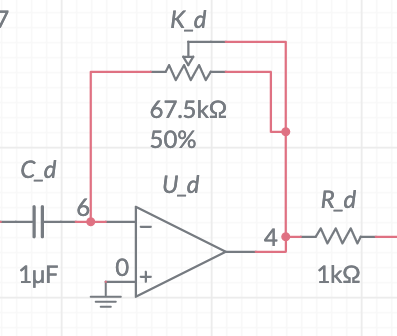
\includegraphics[width = 0.5\textwidth]{opam as differencit.png}
	\caption{OPAMP as a differentiator}
\end{figure}

\subsection{Derivation of Op-amp as Differentiator}
As shown in the figure, a connection of capacitor in series with the input voltage source has been made. The input capacitor $C_{1}$ is initially uncharged and hence operate as an open-circuit. The non-inverting terminal of the amplifier is connected to the ground, whereas the inverting input terminal is through the negative feedback resistor $\mathrm{R}_{\mathrm{f}}$ and connected to output terminal.

Due to the ideal op-amp characteristics (the input impedance of the op-amp is infinite) as the input current, I to the input of an op-amp is ideally zero. Therefore the current flowing through the capacitor (in this configuration, the input resistance is replaced by a capacitor) due to the applied input voltage $\mathrm{V}_{\text {in }}$ flows along the feedback path through the feedback resistor $\mathrm{R}_{\mathrm{f}}$.
As observed from the figure, point $\mathrm{X}$ is virtually grounded (according to the virtual ground concept) because the non-inverting input terminal is grounded (point $Y$ is at ground potential i.e., $0 \mathrm{~V}$ ).
Consequently, $\mathrm{Vx}=\mathrm{Vy}=0$
With respect to the input side capacitor, the current carrying through the capacitor can be written as:
$$
\mathrm{I}=\mathrm{c}_{1} \frac{\mathrm{d}\left(\mathrm{V}_{\mathrm{in}}-\mathrm{V}_{\mathrm{X}}\right)}{\mathrm{dt}}=\frac{\mathrm{c}_{1} \mathrm{~d}\left(\mathrm{~V}_{\text {in }}\right)}{\mathrm{dt}}
$$
With respect to the output side feedback resistor, the current flowing through it can be represented as:
$$
1=\frac{V_{x}-V_{0}}{R_{f}}=-\frac{V_{0}}{R_{f}}
$$
From the above equations when we equate the currents in both the results we get,
$$
\begin{gathered}
\frac{c_{1} d\left(v_{i n}\right)}{d t}=-\frac{v_{0}}{R_{f}} \\
V_{0}=-C_{1} R_{f} \frac{d\left(V_{i n}\right)}{d t}
\end{gathered}
$$
The differentiating amplifier circuit requires a very small time constant for its application (differentiation), and hence it is one of its main advantages.
The product value $C_{1} R_{f}$ is known as differentiator's time constant, and output of the differentiator is $C_{1} R_{f}$ times the differentiation of $\mathrm{V}_{\text {in }}$ signal. The -ve sign in the equation refers that the output is $180^{\circ}$ difference in phase with reference to the input.
When we apply a constant voltage with one step change at $\mathrm{t}=0$ like a step signal in the input terminal of the differentiator, the output should be ideally zero as the differentiation of constant is zero. But in practice, the output is not exactly zero because the constant input wave takes some amount of time to step from 0 volts to some $\mathrm{V}_{\max }$ volts. Therefore the output waveform appears to have a spike at time $\mathrm{t}=0 .$






\section{Observation and Calculations}


\newcommand{\plott}[3]{
\subsubsection{Seting the values of $K_p = \to \text{#1} K_p$ , $K_i \to \text{#2} K_i $ $K_d \to \text{#3} K_d$ we get the plot.}
\begin{figure}[H]
    \includegraphics[width= \linewidth]{PID-(#1,#2,#3).png}
    \caption{PID(#1,#2,#3)}{
    }
\end{figure}
}
\plott{}{}{}
\plott{2x}{}{}
\plott{}{2x}{}
\plott{}{}{2x}

\setcounter{equation}{0}
\setcounter{table}{0}
\setcounter{figure}{0}
%\baselineskip 24pt


    



